```latex
\documentclass[11pt, a4paper]{article}
\usepackage[utf8]{inputenc}
\usepackage[T1]{fontenc}
\usepackage{lmodern}
\usepackage{amsmath, amssymb}
\usepackage{booktabs}
\usepackage{tabularx}
\usepackage{geometry}
\geometry{margin=1in}
\usepackage{minted}
\usepackage[framemethod=TikZ]{mdframed}
\usepackage{tikz}
\usetikzlibrary{shapes.geometric, arrows.meta, positioning}

% Custom command for critical exam-relevant remarks
\newcommand{\sta}{\textbf{[*] }}

% Custom environment for important definitions and theorems
\newmdenv[
    backgroundcolor=gray!10,
    linecolor=black,
    linewidth=1pt,
    roundcorner=4pt,
    innertopmargin=10pt,
    innerbottommargin=10pt,
    innerleftmargin=10pt,
    innerrightmargin=10pt,
]{important}

\begin{document}
% Lecture Notes: Foundations of DNA Sequencing Technology and Genome Assembly

\section{Introduction to Bioinformatics}

Bioinformatics is an interdisciplinary field that combines concepts from molecular biology, computer science, and mathematics/statistics. To properly process and interpret biological data, a bioinformatician must understand the underlying biological mechanisms that generate the data, the algorithms used to analyze it, and the statistical methods required to prove the validity of predictions.

\begin{important}
    \textbf{Bioinformatics}: The application of computational, mathematical, and statistical methods to analyze, store, manipulate, and classify biological information, particularly large and complex datasets like DNA and amino acid sequences.
\end{important}

When analyzing biological systems, we frequently encounter three distinct experimental contexts:
\begin{itemize}
    \item \textbf{\textit{In vivo}}: Processes occurring within a living organism.
    \item \textbf{\textit{In vitro}}: Processes occurring in an artificial environment outside a living organism, such as a glass petri dish or test tube.
    \item \textbf{\textit{In silico}}: Processes performed via computer simulation or computational analysis (derived from "silicon" microchips).
\end{itemize}

\section{Molecular Biology Basics}

To meaningfully work with genomic data, we must understand how biological information is stored, replicated, and expressed at the molecular level.

\subsection{Cellular Organization}

Biological organisms are composed of cells, which fundamentally differ in how their genetic material is organized. In \textbf{prokaryotic cells} (e.g., bacteria), the DNA is organized as a single circular genome freely floating in the cytoplasm. In contrast, \textbf{eukaryotic cells} (e.g., animal and plant cells) store their DNA inside a specialized organelle called the nucleus, packaged into individual molecules called chromosomes.

This physical separation in eukaryotes—storing genetic blueprints in the nucleus while protein production occurs outside it—allows for complex post-processing of genetic messages, a feature prokaryotes lack. 

\subsection{Nucleic Acids: DNA and RNA}

The primary macromolecules responsible for genetic information are DNA and RNA. Both are polymers constructed from individual monomer units called nucleotides.

\begin{important}
    \textbf{Deoxyribonucleic Acid (DNA)}: A double-stranded helical molecule that stores the primary genetic information of a cell. 
    
    \textbf{Ribonucleic Acid (RNA)}: A primarily single-stranded molecule involved in translating genetic information from DNA into functional proteins, and regulating cellular processes.
\end{important}

% [IMAGE: Diagram showing the chemical structure of a nucleotide: a central pentose sugar attached to a phosphate group at the 5' carbon, and a nitrogenous base attached to the 1' carbon.]

Each nucleotide building block consists of three components:
\begin{enumerate}
    \item A \textbf{pentose sugar} (5-carbon sugar).
    \item At least one \textbf{phosphate group} attached to the 5' (five-prime) carbon of the sugar.
    \item A \textbf{nitrogenous base}, which determines the specific identity of the nucleotide.
\end{enumerate}

Nucleotides form a polymer chain by binding the phosphate group of one nucleotide to the 3' (three-prime) carbon of the next nucleotide. This creates an alternating sugar-phosphate \textbf{backbone} and gives the molecule a strict directionality. By biological convention, we always read sequences from the free \textbf{5' end} to the free \textbf{3' end}.

\begin{table}[h!]
    \centering
    \caption{Key Structural Differences Between DNA and RNA}
    \begin{tabularx}{\textwidth}{l X X}
        \toprule
        \textbf{Feature} & \textbf{DNA} & \textbf{RNA} \\
        \midrule
        \textbf{Sugar Type} & Deoxyribose (lacks one oxygen atom at the 2' carbon) & Ribose \\
        \textbf{Strand Structure} & Double-stranded (Double Helix) & Single-stranded (can form complex 3D shapes via self-pairing) \\
        \textbf{Nitrogenous Bases} & Adenine (A), Cytosine (C), Guanine (G), Thymine (T) & Adenine (A), Cytosine (C), Guanine (G), Uracil (U) \\
        \bottomrule
    \end{tabularx}
\end{table}

\subsection{Base Pairing and the Reverse Complement}

In DNA, the two strands wrap around each other in a double helix. They are held together by the chemical attraction between specific pairs of nitrogenous bases. Adenine (A) always pairs with Thymine (T), and Cytosine (C) always pairs with Guanine (G). 

Crucially, the two strands run in opposite directions (antiparallel). If one strand runs 5' to 3', the opposing strand runs 3' to 5'. 

\begin{important}
    \textbf{Reverse Complement}: The sequence of the opposing DNA strand. It is generated by reversing the reading direction of the original sequence and substituting each base with its complement (A $\leftrightarrow$ T, C $\leftrightarrow$ G).
\end{important}

\textbf{Example:} Generating a Reverse Complement
\begin{itemize}
    \item Positive Strand (5' to 3'): \texttt{A-G-T-C}
    \item Complement (A$\to$T, G$\to$C, T$\to$A, C$\to$G): \texttt{T-C-A-G}
    \item \textbf{Reverse Complement} (read backwards, 5' to 3'): \texttt{G-A-C-T}
\end{itemize}
This process illustrates that knowing the sequence of one strand provides the exact sequence of the other strand.

\sta This property is biologically essential for cell division (DNA replication), as separating the strands provides two perfect templates. Computationally, it is just as vital: when bioinformaticians search a reference genome for a specific sequence pattern, they must always search for both the sequence \textit{and} its reverse complement, as biological features (like genes or protein binding sites) can appear on either strand.

\subsection{The Central Dogma of Molecular Biology}

The flow of genetic information in a cell roughly follows a framework known as the Central Dogma, moving from storage to functional molecular machinery.

\begin{center}
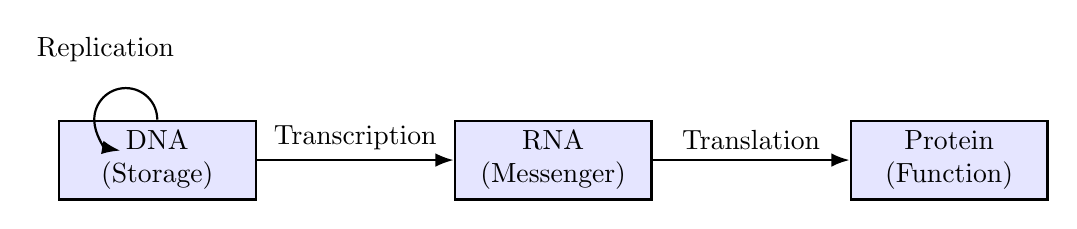
\begin{tikzpicture}[
    node distance=2.5cm,
    box/.style={rectangle, draw=black, thick, fill=blue!10, minimum width=2.5cm, minimum height=1cm, align=center},
    arrow/.style={-Latex, thick}
]
    % Nodes
    \node[box] (dna) {DNA\\(Storage)};
    \node[box, right=of dna] (rna) {RNA\\(Messenger)};
    \node[box, right=of rna] (protein) {Protein\\(Function)};

    % Arrows
    \draw[arrow] (dna) -- node[above] {Transcription} (rna);
    \draw[arrow] (rna) -- node[above] {Translation} (protein);
    \draw[arrow] (dna.north) arc[start angle=0, end angle=260, radius=0.4cm] node[midway, above=0.3cm] {Replication};
\end{tikzpicture}
\end{center}

\begin{enumerate}
    \item \textbf{Transcription}: A specific region of DNA (a gene) is opened, and one strand is copied into a matching RNA sequence (Messenger RNA, or mRNA).
    \item \textbf{Alternative Splicing} (Eukaryotes only): Before the mRNA leaves the nucleus, segments called \textit{introns} are cut out and discarded. The remaining segments, \textit{exons}, are stitched together. A cell can dynamically choose which exons to include or skip, allowing a single gene to produce multiple varying proteins depending on the cell's current needs.
    \item \textbf{Translation}: Outside the nucleus, a complex called a ribosome reads the mRNA sequence and builds a specific protein. 
\end{enumerate}

Proteins are polymers of \textbf{amino acids} (there are 20 standard amino acids). Because there are only 4 RNA bases (A, C, G, U) but 20 amino acids, the ribosome reads the RNA in triplets called \textbf{codons}. 
There are \(4^3 = 64\) possible codons. This introduces redundancy into the genetic code (e.g., multiple codons code for the same amino acid). Specific codons designate the "start" (initiating translation) and "stop" (terminating the protein chain).

\section{DNA Sequencing Technologies}

Sequencing is the process of determining the exact order of nucleotides in a DNA molecule. Knowing the molecular mechanics of the cell allows us to exploit them in the laboratory to read DNA. 

\subsection{Sanger Sequencing (First Generation)}

Developed by Fred Sanger, this highly accurate technique relies on the principle of "sequencing by synthesis"—reconstructing the reverse complement strand and observing what gets inserted.

\begin{important}
    \textbf{Chain-Terminating Dideoxynucleotides}: Artificially modified nucleotides used in Sanger sequencing that lack an oxygen atom at the 3' carbon. When a cell's DNA polymerase inserts one of these, it physically cannot attach the next nucleotide, terminating the chain's growth.
\end{important}

\textbf{The Sanger Sequencing Process:}
\begin{enumerate}
    \item The target DNA is separated into single strands.
    \item The sample is mixed with DNA polymerase, normal nucleotides, and a small amount of fluorescently labeled chain-terminating nucleotides (e.g., A is green, T is red, C is blue, G is yellow).
    \item The polymerase begins synthesizing the reverse complement. Eventually, by random chance, it incorporates a terminating nucleotide, stopping the process. Over many reactions, this creates a pool of DNA fragments of every possible length.
    \item The fragments are passed through an electrophoretic gel. Smaller fragments travel faster than larger ones.
    \item A laser reads the fluorescent color of each fragment as it passes. 
\end{enumerate}

By observing the sequence of colors ordered by fragment size, the sequence is perfectly revealed. While Sanger sequencing is incredibly accurate, its throughput is very low. It was the primary technology used to sequence the first draft of the Human Genome in 2001 (a \$100 million international effort taking roughly 45,000 runs to achieve a \(6\times\) coverage).

% [IMAGE: A chromatogram showing peaks of different colors (red, green, blue, yellow) mapped over time/fragment length, illustrating how the DNA sequence is read base-by-base in Sanger sequencing.]

\subsection{Next Generation Sequencing (NGS / Illumina)}

To sequence billions of bases quickly and affordably (under \$1,000 for a human genome today), "Next Generation Sequencing" massively parallels the synthesis process.

\begin{important}
    \textbf{Bridge Amplification}: A localized PCR-like process on a glass flow cell that duplicates a single DNA fragment thousands of times in a tiny physical cluster. This cluster provides a strong, unified fluorescent signal that a camera can easily read.
\end{important}

\textbf{The NGS Workflow:}
\begin{enumerate}
    \item \textbf{Library Preparation}: Genomic DNA is shattered into millions of random small fragments ("shotgun sequencing"). Known synthetic DNA sequences called \textbf{adapters} are chemically glued to the 5' and 3' ends of every fragment.
    \item \textbf{Flow Cell Binding}: The fragments are washed over a glass slide (flow cell) coated with sequences complementary to the adapters. The fragments hybridize (stick) to the slide.
    \item \textbf{Bridge Amplification}: The fragments are bent over and copied repeatedly, creating millions of distinct "clusters" on the slide. Each cluster contains thousands of identical copies of one original random DNA fragment.
    \item \textbf{Massively Parallel Sequencing by Synthesis}: 
    \begin{itemize}
        \item Modified nucleotides with a temporary "blocker" and a fluorescent dye are washed over the slide.
        \item Polymerase adds exactly \textit{one} nucleotide to every sequence in every cluster. The blocker prevents further additions.
        \item A camera flashes a laser and records the color emitted by every cluster simultaneously.
        \item The blockers and dyes are chemically washed away, and the cycle repeats.
    \end{itemize}
\end{enumerate}

\textbf{Limitations of NGS (Short Reads):}
Because the addition of nucleotides relies on stochastic biochemical reactions, occasionally a sequence in a cluster misses a cycle or adds two bases. Over many cycles (bases), the fragments within a single cluster fall out of sync. This "mixed signal" degrades the optical quality over time, limiting NGS read lengths to relatively short sequences (e.g., 150 to 500 base pairs). 

Computationally, this leaves the bioinformatician with millions of tiny puzzle pieces ("reads") that must be computationally mapped against a 3-billion-base reference genome—a problem known as \textbf{Read Mapping} or \textbf{Genome Assembly}.

\subsection{Third Generation Sequencing (Long Read)}

To resolve the issue of short reads, particularly when assembling highly repetitive genomic regions, third-generation sequencing was developed. 

\begin{important}
    \textbf{Nanopore Sequencing}: A third-generation technology where a single DNA molecule is pulled through a microscopic pore in a membrane. As the molecule passes through, each base disrupts an applied electrical current uniquely. By recording the current fluctuations, the sequence is interpreted.
\end{important}

Nanopore technologies allow for incredibly long reads (10,000 to 100,000+ bases). Historically, they suffered from higher error rates (\(\sim 10\%\)) compared to NGS, but algorithmic and chemical improvements have vastly increased their accuracy over time.

\subsection{Applications of Sequencing Technologies}

While these machines read DNA, biochemical cleverness allows them to profile almost any level of cellular biology:
\begin{itemize}
    \item \textbf{Genomics} (DNA-Seq): Sequencing standard DNA to find mutations, variants, or assemble new species.
    \item \textbf{Transcriptomics} (RNA-Seq): Capturing mRNA, copying it backward into complementary DNA (cDNA), and sequencing it to measure how actively specific genes are expressed under varying conditions.
    \item \textbf{Protein-DNA Interactions} (ChIP-Seq): Using chemicals to "freeze" (cross-link) proteins attached to DNA, isolating the complex, and sequencing the attached DNA fragments to locate exactly where in the genome specific regulatory proteins bind.
\end{itemize}

\sta \textit{Garbage in, Garbage out}: As a bioinformatician, understanding the experimental source and inherent physical limitations of these sequencing technologies is crucial. High-throughput data carries inherent error rates and quality scores. Processing this data without respecting the noise profile of the sequencing machine will yield fundamentally flawed biological insights.

\end{document}
```